% Options for packages loaded elsewhere
\PassOptionsToPackage{unicode}{hyperref}
\PassOptionsToPackage{hyphens}{url}
%
\documentclass[
]{article}
\usepackage{amsmath,amssymb}
\usepackage{lmodern}
\usepackage{iftex}
\ifPDFTeX
  \usepackage[T1]{fontenc}
  \usepackage[utf8]{inputenc}
  \usepackage{textcomp} % provide euro and other symbols
\else % if luatex or xetex
  \usepackage{unicode-math}
  \defaultfontfeatures{Scale=MatchLowercase}
  \defaultfontfeatures[\rmfamily]{Ligatures=TeX,Scale=1}
\fi
% Use upquote if available, for straight quotes in verbatim environments
\IfFileExists{upquote.sty}{\usepackage{upquote}}{}
\IfFileExists{microtype.sty}{% use microtype if available
  \usepackage[]{microtype}
  \UseMicrotypeSet[protrusion]{basicmath} % disable protrusion for tt fonts
}{}
\makeatletter
\@ifundefined{KOMAClassName}{% if non-KOMA class
  \IfFileExists{parskip.sty}{%
    \usepackage{parskip}
  }{% else
    \setlength{\parindent}{0pt}
    \setlength{\parskip}{6pt plus 2pt minus 1pt}}
}{% if KOMA class
  \KOMAoptions{parskip=half}}
\makeatother
\usepackage{xcolor}
\usepackage[margin=1in]{geometry}
\usepackage{color}
\usepackage{fancyvrb}
\newcommand{\VerbBar}{|}
\newcommand{\VERB}{\Verb[commandchars=\\\{\}]}
\DefineVerbatimEnvironment{Highlighting}{Verbatim}{commandchars=\\\{\}}
% Add ',fontsize=\small' for more characters per line
\usepackage{framed}
\definecolor{shadecolor}{RGB}{248,248,248}
\newenvironment{Shaded}{\begin{snugshade}}{\end{snugshade}}
\newcommand{\AlertTok}[1]{\textcolor[rgb]{0.94,0.16,0.16}{#1}}
\newcommand{\AnnotationTok}[1]{\textcolor[rgb]{0.56,0.35,0.01}{\textbf{\textit{#1}}}}
\newcommand{\AttributeTok}[1]{\textcolor[rgb]{0.77,0.63,0.00}{#1}}
\newcommand{\BaseNTok}[1]{\textcolor[rgb]{0.00,0.00,0.81}{#1}}
\newcommand{\BuiltInTok}[1]{#1}
\newcommand{\CharTok}[1]{\textcolor[rgb]{0.31,0.60,0.02}{#1}}
\newcommand{\CommentTok}[1]{\textcolor[rgb]{0.56,0.35,0.01}{\textit{#1}}}
\newcommand{\CommentVarTok}[1]{\textcolor[rgb]{0.56,0.35,0.01}{\textbf{\textit{#1}}}}
\newcommand{\ConstantTok}[1]{\textcolor[rgb]{0.00,0.00,0.00}{#1}}
\newcommand{\ControlFlowTok}[1]{\textcolor[rgb]{0.13,0.29,0.53}{\textbf{#1}}}
\newcommand{\DataTypeTok}[1]{\textcolor[rgb]{0.13,0.29,0.53}{#1}}
\newcommand{\DecValTok}[1]{\textcolor[rgb]{0.00,0.00,0.81}{#1}}
\newcommand{\DocumentationTok}[1]{\textcolor[rgb]{0.56,0.35,0.01}{\textbf{\textit{#1}}}}
\newcommand{\ErrorTok}[1]{\textcolor[rgb]{0.64,0.00,0.00}{\textbf{#1}}}
\newcommand{\ExtensionTok}[1]{#1}
\newcommand{\FloatTok}[1]{\textcolor[rgb]{0.00,0.00,0.81}{#1}}
\newcommand{\FunctionTok}[1]{\textcolor[rgb]{0.00,0.00,0.00}{#1}}
\newcommand{\ImportTok}[1]{#1}
\newcommand{\InformationTok}[1]{\textcolor[rgb]{0.56,0.35,0.01}{\textbf{\textit{#1}}}}
\newcommand{\KeywordTok}[1]{\textcolor[rgb]{0.13,0.29,0.53}{\textbf{#1}}}
\newcommand{\NormalTok}[1]{#1}
\newcommand{\OperatorTok}[1]{\textcolor[rgb]{0.81,0.36,0.00}{\textbf{#1}}}
\newcommand{\OtherTok}[1]{\textcolor[rgb]{0.56,0.35,0.01}{#1}}
\newcommand{\PreprocessorTok}[1]{\textcolor[rgb]{0.56,0.35,0.01}{\textit{#1}}}
\newcommand{\RegionMarkerTok}[1]{#1}
\newcommand{\SpecialCharTok}[1]{\textcolor[rgb]{0.00,0.00,0.00}{#1}}
\newcommand{\SpecialStringTok}[1]{\textcolor[rgb]{0.31,0.60,0.02}{#1}}
\newcommand{\StringTok}[1]{\textcolor[rgb]{0.31,0.60,0.02}{#1}}
\newcommand{\VariableTok}[1]{\textcolor[rgb]{0.00,0.00,0.00}{#1}}
\newcommand{\VerbatimStringTok}[1]{\textcolor[rgb]{0.31,0.60,0.02}{#1}}
\newcommand{\WarningTok}[1]{\textcolor[rgb]{0.56,0.35,0.01}{\textbf{\textit{#1}}}}
\usepackage{longtable,booktabs,array}
\usepackage{calc} % for calculating minipage widths
% Correct order of tables after \paragraph or \subparagraph
\usepackage{etoolbox}
\makeatletter
\patchcmd\longtable{\par}{\if@noskipsec\mbox{}\fi\par}{}{}
\makeatother
% Allow footnotes in longtable head/foot
\IfFileExists{footnotehyper.sty}{\usepackage{footnotehyper}}{\usepackage{footnote}}
\makesavenoteenv{longtable}
\usepackage{graphicx}
\makeatletter
\def\maxwidth{\ifdim\Gin@nat@width>\linewidth\linewidth\else\Gin@nat@width\fi}
\def\maxheight{\ifdim\Gin@nat@height>\textheight\textheight\else\Gin@nat@height\fi}
\makeatother
% Scale images if necessary, so that they will not overflow the page
% margins by default, and it is still possible to overwrite the defaults
% using explicit options in \includegraphics[width, height, ...]{}
\setkeys{Gin}{width=\maxwidth,height=\maxheight,keepaspectratio}
% Set default figure placement to htbp
\makeatletter
\def\fps@figure{htbp}
\makeatother
\setlength{\emergencystretch}{3em} % prevent overfull lines
\providecommand{\tightlist}{%
  \setlength{\itemsep}{0pt}\setlength{\parskip}{0pt}}
\setcounter{secnumdepth}{-\maxdimen} % remove section numbering
\ifLuaTeX
  \usepackage{selnolig}  % disable illegal ligatures
\fi
\IfFileExists{bookmark.sty}{\usepackage{bookmark}}{\usepackage{hyperref}}
\IfFileExists{xurl.sty}{\usepackage{xurl}}{} % add URL line breaks if available
\urlstyle{same} % disable monospaced font for URLs
\hypersetup{
  pdftitle={Testat 1},
  pdfauthor={Gruppe 1: Jan Hoffmann, Jannis Seefeld, Rabea Götz},
  hidelinks,
  pdfcreator={LaTeX via pandoc}}

\title{Testat 1}
\author{Gruppe 1: Jan Hoffmann, Jannis Seefeld, Rabea Götz}
\date{}

\begin{document}
\maketitle

\hypertarget{eigenes-histogramm}{%
\section{1 Eigenes Histogramm}\label{eigenes-histogramm}}

Es soll ein eigenes Histogramm erzeugt werden. Der Dateiname für das
Skript ist \texttt{myhistogram.R}.

\hypertarget{funktion-myhistogram}{%
\subsection{\texorpdfstring{Funktion
\texttt{myhistogram}}{Funktion myhistogram}}\label{funktion-myhistogram}}

Programmieren Sie in R die Funktion \texttt{myhistogram}, die als
Parameter \texttt{x} einen Vektor aus Zahlen erhält. Die Zahlen werden
in \texttt{n} Intervalle einsortiert, und es wird gezählt, wie oft eine
Zahl in einem Intervall vorkommt. Der Rückgabewert ist eine Liste mit
den Einträgen \texttt{borders}, die die \(n+1\) Intervallgrenzen
enthalten und \texttt{counts}, der die Anzahlen enthält.

\begin{itemize}
\tightlist
\item
  Die \(n\) Intervalle sollen gleich groß sein (\(\Delta b\)), d.h. für
  die Intervallgrenzen \(b_1, b_2, \ldots, b_{n+1}\) gilt
  \(\frac{b_{i+1}-b_{i}}{n}=\Delta b\) für \(i=1, 2, \ldots n\).
\item
  Die äußeren Grenzen \(b_1\) und \(b_n\) sollen als optionale
  Parametern \texttt{min} und \texttt{max} an die Funktion übergeben
  werden. Werte aus \texttt{x}, die zu keinem Intervall gehören, sollen
  ignoriert werden. Es wird aber eine Warnung ausgegeben, die sagt,
  welche Zahlen außerhalb des Bereichs liegen.
\item
  Eine Zahl \(z\) gehört zum \(i\)-ten Intervall, falls
  \(b_i \leq z < b_{i+1}\) gilt.
\end{itemize}

Bis auf \texttt{x} sollen alle Parameter optional sein. Überlegen Sie
sinnvolle Default-Werte.

Es ist natürlich \textbf{nicht} erlaubt, in der eigenen Funktion andere
Funktionen zu nutzen, die ein Histogramm erzeugen.

\begin{Shaded}
\begin{Highlighting}[]
\NormalTok{myhistogram }\OtherTok{=} \ControlFlowTok{function}\NormalTok{(x, }\AttributeTok{n=}\DecValTok{30}\NormalTok{, }\AttributeTok{min=}\ConstantTok{NA}\NormalTok{, }\AttributeTok{max=}\ConstantTok{NA}\NormalTok{) \{}
\NormalTok{    sorted }\OtherTok{=} \FunctionTok{sort}\NormalTok{(x)}
\NormalTok{    min}\OtherTok{=}\FunctionTok{ifelse}\NormalTok{(}\FunctionTok{is.na}\NormalTok{(min), }\FunctionTok{min}\NormalTok{(x), min)}
\NormalTok{    max}\OtherTok{=}\FunctionTok{ifelse}\NormalTok{(}\FunctionTok{is.na}\NormalTok{(max), }\FunctionTok{max}\NormalTok{(x) }\SpecialCharTok{+} \DecValTok{1}\NormalTok{, max)}

\NormalTok{    sortedNumbers }\OtherTok{=}\NormalTok{ sorted[sorted }\SpecialCharTok{\textgreater{}=}\NormalTok{ min]}
\NormalTok{    sortedNumbers }\OtherTok{=}\NormalTok{ sortedNumbers[sortedNumbers }\SpecialCharTok{\textless{}}\NormalTok{ max]}

\NormalTok{    outside }\OtherTok{=}\NormalTok{ sorted[sorted }\SpecialCharTok{\textless{}}\NormalTok{ min]}
\NormalTok{    outside }\OtherTok{=}\NormalTok{ sorted[sorted }\SpecialCharTok{\textgreater{}}\NormalTok{ max]}

    \ControlFlowTok{if}\NormalTok{ (}\FunctionTok{length}\NormalTok{(outside) }\SpecialCharTok{\textgreater{}} \DecValTok{0}\NormalTok{) \{}
        \FunctionTok{warning}\NormalTok{(}\FunctionTok{paste0}\NormalTok{(}\StringTok{\textquotesingle{}Zahlen außerhalb von Intervallgrenzen: \textquotesingle{}}\NormalTok{, }\FunctionTok{paste}\NormalTok{(outside, }\AttributeTok{collapse =} \StringTok{", "}\NormalTok{)))}
\NormalTok{    \}}

\NormalTok{    borders }\OtherTok{=} \FunctionTok{seq}\NormalTok{(min, max, }\AttributeTok{length.out=}\NormalTok{n}\SpecialCharTok{+}\DecValTok{1}\NormalTok{)}
\NormalTok{    counts }\OtherTok{=} \FunctionTok{sapply}\NormalTok{(}\FunctionTok{seq}\NormalTok{(}\AttributeTok{from=}\DecValTok{1}\NormalTok{, }\AttributeTok{to=}\NormalTok{n), }\ControlFlowTok{function}\NormalTok{(e) \{}
\NormalTok{        min }\OtherTok{=}\NormalTok{ borders[e]}
\NormalTok{        max }\OtherTok{=}\NormalTok{ borders[e}\SpecialCharTok{+}\DecValTok{1}\NormalTok{]}

\NormalTok{        intervall }\OtherTok{=}\NormalTok{ sortedNumbers[sortedNumbers }\SpecialCharTok{\textgreater{}=}\NormalTok{ min]}
\NormalTok{        intervall }\OtherTok{=}\NormalTok{ intervall[intervall }\SpecialCharTok{\textless{}}\NormalTok{ max]}

        \FunctionTok{length}\NormalTok{(intervall)}
\NormalTok{    \})}

    \FunctionTok{list}\NormalTok{(borders, counts)}
\NormalTok{\}}
\end{Highlighting}
\end{Shaded}

\hypertarget{beispieldaten}{%
\subsection{2.1 Beispieldaten}\label{beispieldaten}}

\hypertarget{beispiel-1}{%
\subsubsection{1.2.1 Beispiel 1}\label{beispiel-1}}

Es wird eine Warnung ausgeben:

Warning in myhistogram(x, n = 10, min = -5, max = 6): Zahl(en) außerhalb
Intervallgrenzen: 6

\begin{Shaded}
\begin{Highlighting}[]
\NormalTok{x }\OtherTok{=} \FunctionTok{seq}\NormalTok{(}\SpecialCharTok{{-}}\DecValTok{5}\NormalTok{, }\DecValTok{6}\NormalTok{, }\AttributeTok{by =} \DecValTok{1} \SpecialCharTok{/} \DecValTok{3}\NormalTok{)}
\FunctionTok{myhistogram}\NormalTok{(x, }\AttributeTok{n =} \DecValTok{10}\NormalTok{, }\AttributeTok{min =} \SpecialCharTok{{-}}\DecValTok{5}\NormalTok{, }\AttributeTok{max =} \DecValTok{6}\NormalTok{)}
\end{Highlighting}
\end{Shaded}

\begin{verbatim}
## [[1]]
##  [1] -5.0 -3.9 -2.8 -1.7 -0.6  0.5  1.6  2.7  3.8  4.9  6.0
## 
## [[2]]
##  [1] 4 3 3 4 3 3 4 3 3 3
\end{verbatim}

\hypertarget{beispiel-2}{%
\subsubsection{1.2.2 Beispiel 2}\label{beispiel-2}}

\begin{Shaded}
\begin{Highlighting}[]
\NormalTok{x }\OtherTok{=} \FunctionTok{seq}\NormalTok{(}\SpecialCharTok{{-}}\DecValTok{5}\NormalTok{, }\DecValTok{6}\NormalTok{, }\AttributeTok{by =} \DecValTok{1} \SpecialCharTok{/} \DecValTok{3}\NormalTok{)}
\FunctionTok{myhistogram}\NormalTok{(x, }\AttributeTok{n =} \DecValTok{5}\NormalTok{, }\AttributeTok{min =} \SpecialCharTok{{-}}\DecValTok{10}\NormalTok{, }\AttributeTok{max =} \DecValTok{10}\NormalTok{)}
\end{Highlighting}
\end{Shaded}

\begin{verbatim}
## [[1]]
## [1] -10  -6  -2   2   6  10
## 
## [[2]]
## [1]  0  9 12 12  1
\end{verbatim}

\hypertarget{beispiel-3}{%
\subsubsection{1.2.3 Beispiel 3}\label{beispiel-3}}

\begin{Shaded}
\begin{Highlighting}[]
\NormalTok{x }\OtherTok{=} \FunctionTok{seq}\NormalTok{(}\SpecialCharTok{{-}}\DecValTok{5}\NormalTok{, }\DecValTok{5}\NormalTok{, }\AttributeTok{by =} \DecValTok{1} \SpecialCharTok{/} \DecValTok{5}\NormalTok{)}
\FunctionTok{myhistogram}\NormalTok{(x, }\AttributeTok{n =} \DecValTok{7}\NormalTok{, }\AttributeTok{min =} \SpecialCharTok{{-}}\DecValTok{10}\NormalTok{, }\AttributeTok{max =} \DecValTok{10}\NormalTok{)}
\end{Highlighting}
\end{Shaded}

\begin{verbatim}
## [[1]]
## [1] -10.000000  -7.142857  -4.285714  -1.428571   1.428571   4.285714   7.142857
## [8]  10.000000
## 
## [[2]]
## [1]  0  4 14 15 14  4  0
\end{verbatim}

\hypertarget{beispiel-4}{%
\subsubsection{1.2.4 Beispiel 4}\label{beispiel-4}}

\begin{Shaded}
\begin{Highlighting}[]
\NormalTok{x }\OtherTok{=} \FunctionTok{seq}\NormalTok{(}\SpecialCharTok{{-}}\DecValTok{100}\NormalTok{, }\DecValTok{100}\NormalTok{, }\AttributeTok{by =} \DecValTok{1}\NormalTok{)}
\FunctionTok{myhistogram}\NormalTok{(x, }\AttributeTok{n =} \DecValTok{15}\NormalTok{)}
\end{Highlighting}
\end{Shaded}

\begin{verbatim}
## [[1]]
##  [1] -100.0  -86.6  -73.2  -59.8  -46.4  -33.0  -19.6   -6.2    7.2   20.6
## [11]   34.0   47.4   60.8   74.2   87.6  101.0
## 
## [[2]]
##  [1] 14 13 14 13 13 14 13 14 13 13 14 13 14 13 13
\end{verbatim}

\hypertarget{beispiel-5}{%
\subsubsection{1.2.5 Beispiel 5}\label{beispiel-5}}

\begin{Shaded}
\begin{Highlighting}[]
\NormalTok{x }\OtherTok{=} \FunctionTok{seq}\NormalTok{(}\SpecialCharTok{{-}}\DecValTok{10}\NormalTok{, }\DecValTok{11}\NormalTok{, }\AttributeTok{by =} \DecValTok{1} \SpecialCharTok{/} \DecValTok{5}\NormalTok{)}
\FunctionTok{myhistogram}\NormalTok{(x, }\AttributeTok{min =} \SpecialCharTok{{-}}\DecValTok{10}\NormalTok{, }\AttributeTok{max =} \DecValTok{10}\NormalTok{)}
\end{Highlighting}
\end{Shaded}

\begin{verbatim}
## Warning in myhistogram(x, min = -10, max = 10): Zahlen außerhalb von
## Intervallgrenzen: 10.2, 10.4, 10.6, 10.8, 11
\end{verbatim}

\begin{verbatim}
## [[1]]
##  [1] -10.0000000  -9.3333333  -8.6666667  -8.0000000  -7.3333333  -6.6666667
##  [7]  -6.0000000  -5.3333333  -4.6666667  -4.0000000  -3.3333333  -2.6666667
## [13]  -2.0000000  -1.3333333  -0.6666667   0.0000000   0.6666667   1.3333333
## [19]   2.0000000   2.6666667   3.3333333   4.0000000   4.6666667   5.3333333
## [25]   6.0000000   6.6666667   7.3333333   8.0000000   8.6666667   9.3333333
## [31]  10.0000000
## 
## [[2]]
##  [1] 4 3 3 4 3 3 4 3 3 4 3 3 4 3 3 4 3 3 4 3 3 4 3 3 4 3 3 4 3 3
\end{verbatim}

\hypertarget{barplot}{%
\subsection{1.3 Barplot}\label{barplot}}

Nutzen Sie Ihre Funktion \texttt{myhistogram} und erzeugen Sie einen
Barplot mit \emph{ggplot}. Die \emph{x}-Achse zeigt dabei die Mitte des
Intervalls und die \emph{y}-Achse die Anzahl der Elemente in dieser
Klasse.

Tipp: Der Parameter \texttt{stat} von \texttt{geom\_bar} ist wichtig.

Vervollständigen Sie den Chunk. Die Kommentare sollen zu Anweisungen
umgewandelt werden:

\begin{Shaded}
\begin{Highlighting}[]
\FunctionTok{library}\NormalTok{(ggplot2)}

\FunctionTok{set.seed}\NormalTok{(}\DecValTok{1}\NormalTok{)}
\NormalTok{x }\OtherTok{=} \FunctionTok{rnorm}\NormalTok{(}\DecValTok{0}\NormalTok{, }\DecValTok{1}\NormalTok{, }\AttributeTok{n =} \DecValTok{1000}\NormalTok{)}
\NormalTok{h }\OtherTok{=} \FunctionTok{myhistogram}\NormalTok{(x, }\AttributeTok{n =} \DecValTok{5}\NormalTok{)}
\NormalTok{i }\OtherTok{=} \FunctionTok{sapply}\NormalTok{(}\FunctionTok{seq}\NormalTok{(}\AttributeTok{from=}\DecValTok{1}\NormalTok{, }\AttributeTok{to=}\FunctionTok{length}\NormalTok{(h[[}\DecValTok{1}\NormalTok{]])}\SpecialCharTok{{-}}\DecValTok{1}\NormalTok{), }\ControlFlowTok{function}\NormalTok{(e) \{}
\NormalTok{        lower }\OtherTok{=}\NormalTok{ h[[}\DecValTok{1}\NormalTok{]][e]}
\NormalTok{        upper }\OtherTok{=}\NormalTok{ h[[}\DecValTok{1}\NormalTok{]][e}\SpecialCharTok{+}\DecValTok{1}\NormalTok{]}

\NormalTok{        (lower }\SpecialCharTok{+}\NormalTok{ upper) }\SpecialCharTok{/} \DecValTok{2}
\NormalTok{    \})}
\NormalTok{df }\OtherTok{=} \FunctionTok{data.frame}\NormalTok{(}\AttributeTok{Intervalls=}\NormalTok{i, }\AttributeTok{Frequencies=}\NormalTok{h[[}\DecValTok{2}\NormalTok{]])}
\FunctionTok{colnames}\NormalTok{(df) }\OtherTok{=} \FunctionTok{c}\NormalTok{(}\StringTok{\textquotesingle{}Intervalls\textquotesingle{}}\NormalTok{, }\StringTok{\textquotesingle{}Frequencies\textquotesingle{}}\NormalTok{)}

\FunctionTok{ggplot}\NormalTok{(df) }\SpecialCharTok{+}
    \FunctionTok{geom\_bar}\NormalTok{(}\FunctionTok{aes}\NormalTok{(}\AttributeTok{x=}\NormalTok{Intervalls, }\AttributeTok{y=}\NormalTok{Frequencies), }\AttributeTok{stat=}\StringTok{"identity"}\NormalTok{, }\AttributeTok{position=}\StringTok{"dodge"}\NormalTok{)}
\end{Highlighting}
\end{Shaded}

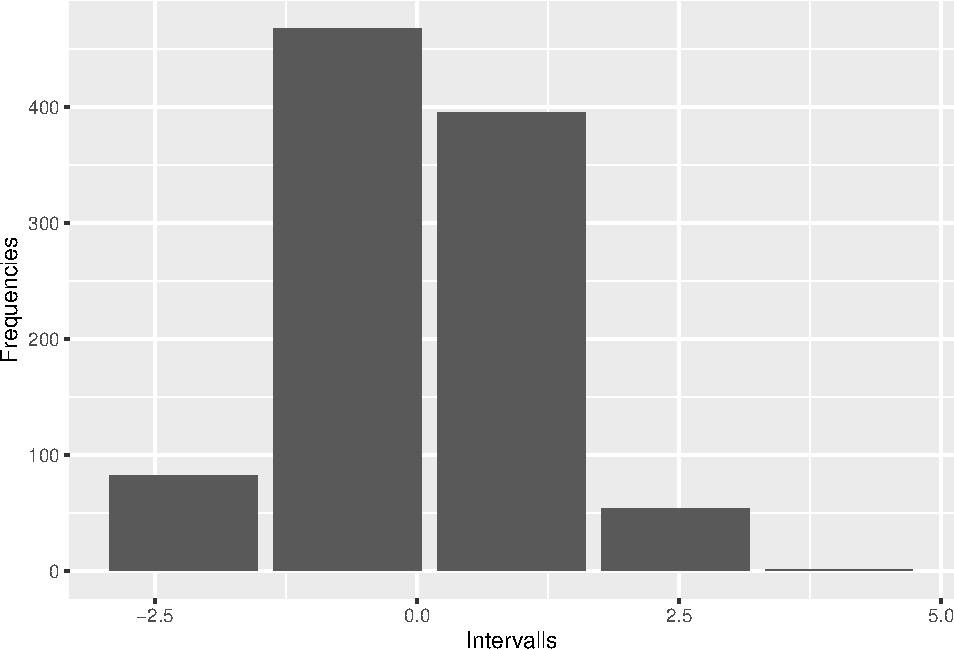
\includegraphics{Testat_1_Complete_files/figure-latex/unnamed-chunk-7-1.pdf}

\hypertarget{visualisierung-von-datensuxe4tzen}{%
\section{2 Visualisierung von
Datensätzen}\label{visualisierung-von-datensuxe4tzen}}

In diesem Abschnitt sollen alle Graphiken mit \emph{ggplot} und alle
Tabellen mit \texttt{kable} erstellt werden.

\hypertarget{kuxf6rpergewicht-und-gehirngewicht-bei-suxe4ugetieren}{%
\subsection{Körpergewicht und Gehirngewicht bei
Säugetieren}\label{kuxf6rpergewicht-und-gehirngewicht-bei-suxe4ugetieren}}

Nutzen Sie den Datensatz \texttt{MASS::mammals}. In der Hilfe finden Sie
Hinweise, was dort gezeigt ist.

\hypertarget{kuxf6rpergewicht-vs.-gehirngewicht}{%
\subsubsection{Körpergewicht
vs.~Gehirngewicht}\label{kuxf6rpergewicht-vs.-gehirngewicht}}

Erzeugen Sie diese Graphik, indem Sie den nachfolgenden Chunk
vervollständigen. Die gezeigten Tiernamen sind Pig, Rat, African
elephant, Chimpanzee, Cat, Human, Little brown bat.

Tipp: Sie dürfen (und sollen) weitere Libraries nutzen, wenn diese
hilfreich sind.

\begin{Shaded}
\begin{Highlighting}[]
\CommentTok{\# Ihre Lösung:}
\NormalTok{mam }\OtherTok{=}\NormalTok{ MASS}\SpecialCharTok{::}\NormalTok{mammals}
\NormalTok{mam}\SpecialCharTok{$}\NormalTok{name }\OtherTok{=} \FunctionTok{row.names}\NormalTok{(mam)}

\NormalTok{lbl }\OtherTok{=} \FunctionTok{c}\NormalTok{(}\StringTok{\textquotesingle{}Pig\textquotesingle{}}\NormalTok{, }\StringTok{\textquotesingle{}Rat\textquotesingle{}}\NormalTok{, }\StringTok{\textquotesingle{}African elephant\textquotesingle{}}\NormalTok{, }\StringTok{\textquotesingle{}Chimpanzee\textquotesingle{}}\NormalTok{, }\StringTok{\textquotesingle{}Cat\textquotesingle{}}\NormalTok{, }\StringTok{\textquotesingle{}Human\textquotesingle{}}\NormalTok{, }\StringTok{\textquotesingle{}Little brown bat\textquotesingle{}}\NormalTok{)}
\NormalTok{lbl\_data }\OtherTok{=}\NormalTok{ mam[mam}\SpecialCharTok{$}\NormalTok{name }\SpecialCharTok{\%in\%}\NormalTok{ lbl,]}

\FunctionTok{ggplot}\NormalTok{(mam) }\SpecialCharTok{+}
 \FunctionTok{geom\_point}\NormalTok{(}\FunctionTok{aes}\NormalTok{(}\AttributeTok{x=}\NormalTok{body, }\AttributeTok{y=}\NormalTok{brain)) }\SpecialCharTok{+}
 \FunctionTok{scale\_y\_continuous}\NormalTok{(}\StringTok{\textquotesingle{}Gehirngewicht (g) \textquotesingle{}}\NormalTok{, }\AttributeTok{trans=}\StringTok{\textquotesingle{}log10\textquotesingle{}}\NormalTok{) }\SpecialCharTok{+}
 \FunctionTok{scale\_x\_continuous}\NormalTok{(}\StringTok{\textquotesingle{}Körpergewicht (kg)\textquotesingle{}}\NormalTok{, }\AttributeTok{trans=}\StringTok{\textquotesingle{}log10\textquotesingle{}}\NormalTok{) }\SpecialCharTok{+}
 \FunctionTok{geom\_text}\NormalTok{(}\FunctionTok{aes}\NormalTok{(}\AttributeTok{label=}\NormalTok{name, }\AttributeTok{x=}\NormalTok{body, }\AttributeTok{y=}\NormalTok{brain),}\AttributeTok{color=}\StringTok{\textquotesingle{}blue\textquotesingle{}}\NormalTok{, }\AttributeTok{data=}\NormalTok{lbl\_data)}
\end{Highlighting}
\end{Shaded}

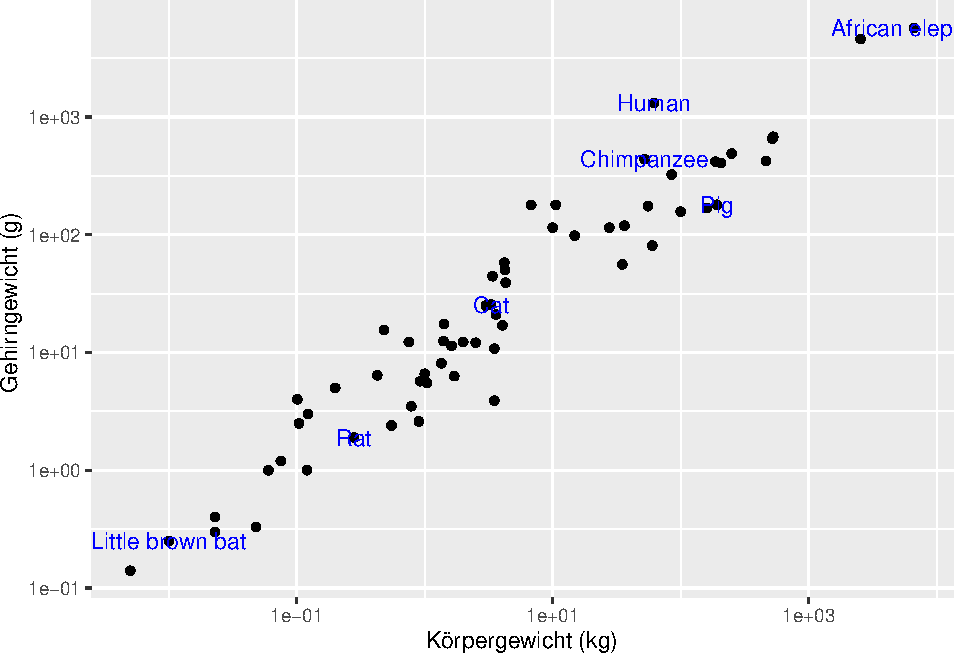
\includegraphics{Testat_1_Complete_files/figure-latex/unnamed-chunk-9-1.pdf}
\#\#\# Gehirn- zu Körpergewicht-Verhältnis

Geben Sie diejenigen 10 Tiere als Tabelle im Notebook aus, die das
größte Gehirn- zu Körpergewicht-Verhältnis \(r\) haben. Die Liste soll
nach \(r\) absteigend sortiert sein und den Tiernamen und \(r\)
enthalten.

Vervollständigen Sie diesen Chunk:

\begin{Shaded}
\begin{Highlighting}[]
\CommentTok{\# Ihre Lösung:}
\NormalTok{mam}\SpecialCharTok{$}\NormalTok{r }\OtherTok{=}\NormalTok{ mam}\SpecialCharTok{$}\NormalTok{brain}\SpecialCharTok{/}\NormalTok{mam}\SpecialCharTok{$}\NormalTok{body}
\FunctionTok{kable}\NormalTok{(}\FunctionTok{head}\NormalTok{(mam[}\FunctionTok{order}\NormalTok{(mam}\SpecialCharTok{$}\NormalTok{r, }\AttributeTok{decreasing=}\NormalTok{T),][}\FunctionTok{c}\NormalTok{(}\DecValTok{4}\NormalTok{)],}\AttributeTok{n=}\DecValTok{10}\NormalTok{))}
\end{Highlighting}
\end{Shaded}

\begin{longtable}[]{@{}lr@{}}
\toprule()
& r \\
\midrule()
\endhead
Ground squirrel & 39.60396 \\
Owl monkey & 32.29167 \\
Lesser short-tailed shrew & 28.00000 \\
Rhesus monkey & 26.32353 \\
Galago & 25.00000 \\
Little brown bat & 25.00000 \\
Mole rat & 24.59016 \\
Tree shrew & 24.03846 \\
Human & 21.29032 \\
Mouse & 17.39130 \\
\bottomrule()
\end{longtable}

Geben Sie nun -- wie eben -- diejenigen 10 Tiere als Tabelle aus, die
das \textbf{kleinste} Gehirn- zu Körpergewicht-Verhältnis \(r\) haben.
Die Liste soll nach \(r\) absteigend sortiert sein.

Vervollständigen Sie diesen Chunk:

\begin{Shaded}
\begin{Highlighting}[]
\CommentTok{\# Ihre Lösung:}
\FunctionTok{kable}\NormalTok{(}\FunctionTok{tail}\NormalTok{(mam[}\FunctionTok{order}\NormalTok{(mam}\SpecialCharTok{$}\NormalTok{r, }\AttributeTok{decreasing=}\NormalTok{T),][}\DecValTok{4}\NormalTok{],}\AttributeTok{n=}\DecValTok{10}\NormalTok{))}
\end{Highlighting}
\end{Shaded}

\begin{longtable}[]{@{}lr@{}}
\toprule()
& r \\
\midrule()
\endhead
Kangaroo & 1.6000000 \\
Jaguar & 1.5700000 \\
Giant armadillo & 1.3500000 \\
Giraffe & 1.2854442 \\
Horse & 1.2571977 \\
Water opossum & 1.1142857 \\
Brazilian tapir & 1.0562500 \\
Pig & 0.9375000 \\
Cow & 0.9096774 \\
African elephant & 0.8584310 \\
\bottomrule()
\end{longtable}

\hypertarget{blutdruckveruxe4nderung-bei-medikamentengabe-im-tierversuch}{%
\subsection{Blutdruckveränderung bei Medikamentengabe im
Tierversuch}\label{blutdruckveruxe4nderung-bei-medikamentengabe-im-tierversuch}}

Nutzen Sie den Datensatz \texttt{MASS::Rabbit}. In der Hilfe finden Sie
Hinweise, was dort gezeigt ist.

\hypertarget{uxfcberblick-uxfcber-verlauf-bei-allen-kaninchen}{%
\subsubsection{Überblick über Verlauf bei allen
Kaninchen}\label{uxfcberblick-uxfcber-verlauf-bei-allen-kaninchen}}

Plotten Sie im folgenden Chunk den Verlauf der Blutdruckveränderung
(\emph{y}-Achse) bei gegebener Dosis Phenylbiguanide (\emph{x}-Achse).
Dies soll in einem Diagramm mit Unterdiagrammen erfolgen: ein
Unterdiagramm zeigt den Verlauf für je ein Kaninchen und der Behandlung
(Placebo oder MDL 72222).

\begin{Shaded}
\begin{Highlighting}[]
\CommentTok{\# Ihre Lösung:}
\FunctionTok{ggplot}\NormalTok{(MASS}\SpecialCharTok{::}\NormalTok{Rabbit) }\SpecialCharTok{+} \FunctionTok{geom\_line}\NormalTok{(}\FunctionTok{aes}\NormalTok{(}\AttributeTok{y=}\NormalTok{BPchange, }\AttributeTok{x=}\NormalTok{Dose)) }\SpecialCharTok{+} \FunctionTok{facet\_grid}\NormalTok{( Treatment}\SpecialCharTok{\textasciitilde{}}\NormalTok{Animal)}
\end{Highlighting}
\end{Shaded}

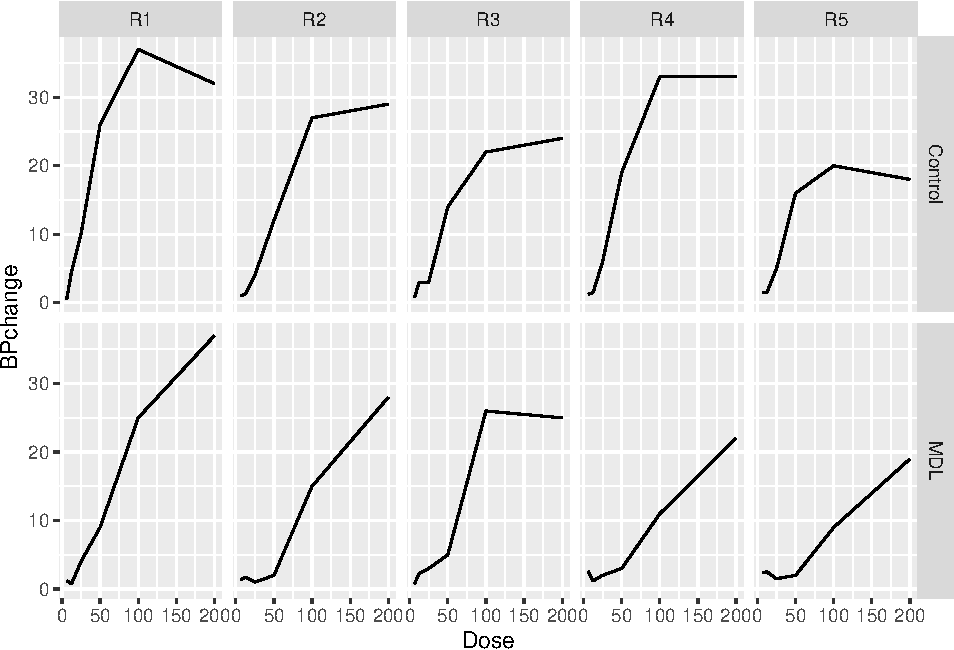
\includegraphics{Testat_1_Complete_files/figure-latex/unnamed-chunk-12-1.pdf}

\hypertarget{boxplots-der-blutdruckuxe4nderung-je-dosis}{%
\subsubsection{Boxplots der Blutdruckänderung je
Dosis}\label{boxplots-der-blutdruckuxe4nderung-je-dosis}}

Erzeugen Sie ein Diagramm, das in zwei Unterdiagrammen für die Placebo-
und die MLD-Gruppe Boxplots erstellt. Die Boxplots geben die Verteilung
der Blutdruckänderung je Dosis an. In Anlehnung an das obige Diagramm
sollen die Boxplots vertikal ausgerichtet sein.

\begin{Shaded}
\begin{Highlighting}[]
\CommentTok{\# Ihre Lösung:}
\FunctionTok{ggplot}\NormalTok{(MASS}\SpecialCharTok{::}\NormalTok{Rabbit) }\SpecialCharTok{+} \FunctionTok{geom\_boxplot}\NormalTok{(}\FunctionTok{aes}\NormalTok{(}\AttributeTok{y=}\NormalTok{BPchange,}\AttributeTok{x=}\FunctionTok{factor}\NormalTok{(Dose), }\AttributeTok{group=}\NormalTok{Dose)) }\SpecialCharTok{+}
  \FunctionTok{xlab}\NormalTok{(}\StringTok{"Dose"}\NormalTok{)}\SpecialCharTok{+}
  \FunctionTok{facet\_wrap}\NormalTok{(}\SpecialCharTok{\textasciitilde{}}\NormalTok{Treatment)}
\end{Highlighting}
\end{Shaded}

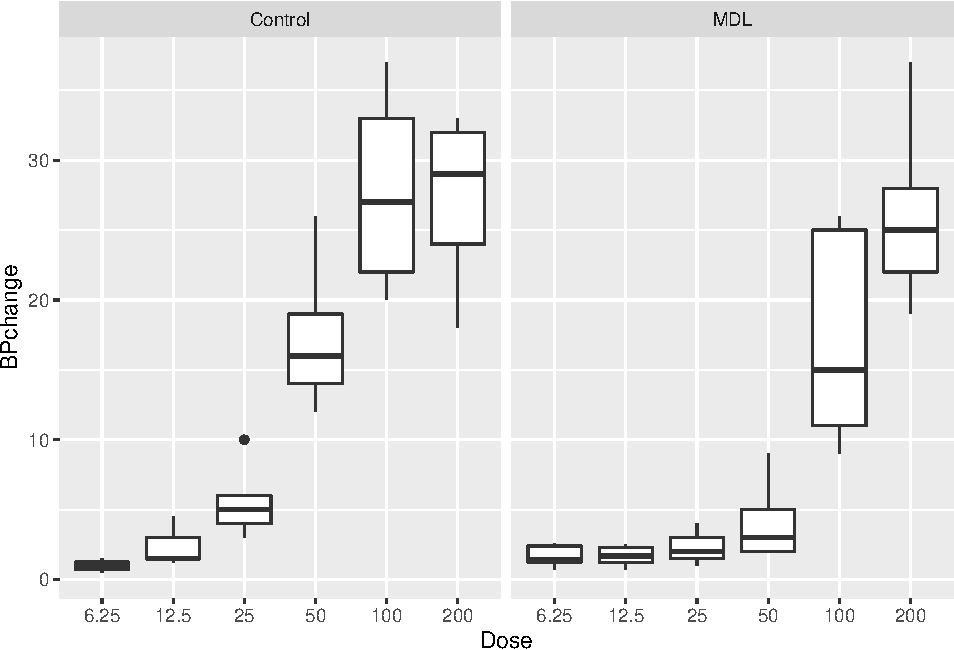
\includegraphics{Testat_1_Complete_files/figure-latex/unnamed-chunk-13-1.pdf}

\hypertarget{covid19-impffortschritt-in-deutschland}{%
\section{3 Covid19: Impffortschritt in
Deutschland}\label{covid19-impffortschritt-in-deutschland}}

In dieser Aufgabe geht es um den Verlauf der Corona-Impfungen in
Deutschland. Die folgenden URLs enthalten Daten ab 2020:

\begin{itemize}
\tightlist
\item
  \url{https://impfdashboard.de/static/data/germany_vaccinations_timeseries_v2.tsv}
\item
  \url{https://impfdashboard.de/static/data/germany_deliveries_timeseries_v2.tsv}
\item
  \url{https://impfdashboard.de/static/data/germany_vaccinations_by_state.tsv}
\end{itemize}

Sie sind der Webseite \url{https://impfdashboard.de} entnommen.

\hypertarget{einlesen-der-daten}{%
\subsection{Einlesen der Daten}\label{einlesen-der-daten}}

Lesen Sie die drei Dateien je in einen Data Frame ein mit den
Variablennamen:

\begin{itemize}
\tightlist
\item
  \texttt{vacc}
\item
  \texttt{deliv}
\item
  \texttt{vaccState}
\end{itemize}

Wandeln Sie die Datums- und Zeitangaben von einem String in ein
R-Datumsobjekt um. Geben Sie die ersten drei Zeilen und Spalten dieser
Data Frames aus.

\begin{Shaded}
\begin{Highlighting}[]
\CommentTok{\# Ihre Lösung:}
\CommentTok{\# germany\_vaccinations\_timeseries\_v2.tsv in Variable vacc}
\CommentTok{\# germany\_deliveries\_timeseries\_v2.tsv in Variable deliv}
\CommentTok{\# germany\_vaccinations\_by\_state.tsv in Variable vaccState}

 
\NormalTok{vacc }\OtherTok{=} \FunctionTok{read.table}\NormalTok{(}\StringTok{\textquotesingle{}https://impfdashboard.de/static/data/germany\_vaccinations\_timeseries\_v2.tsv\textquotesingle{}}\NormalTok{, }
                  \AttributeTok{sep=}\StringTok{\textquotesingle{}}\SpecialCharTok{\textbackslash{}t}\StringTok{\textquotesingle{}}\NormalTok{, }\AttributeTok{header=}\NormalTok{T)}

\NormalTok{deliv }\OtherTok{=} \FunctionTok{read.table}\NormalTok{(}\StringTok{\textquotesingle{}https://impfdashboard.de/static/data/germany\_deliveries\_timeseries\_v2.tsv\textquotesingle{}}\NormalTok{, }
                   \AttributeTok{sep=}\StringTok{\textquotesingle{}}\SpecialCharTok{\textbackslash{}t}\StringTok{\textquotesingle{}}\NormalTok{, }\AttributeTok{header=}\NormalTok{T)}

\NormalTok{vaccState }\OtherTok{=} \FunctionTok{read.table}\NormalTok{(}\StringTok{\textquotesingle{}https://impfdashboard.de/static/data/germany\_vaccinations\_by\_state.tsv\textquotesingle{}}\NormalTok{, }
                       \AttributeTok{sep=}\StringTok{\textquotesingle{}}\SpecialCharTok{\textbackslash{}t}\StringTok{\textquotesingle{}}\NormalTok{, }\AttributeTok{header=}\NormalTok{T)}
 
\NormalTok{deliv}\SpecialCharTok{$}\NormalTok{date }\OtherTok{=} \FunctionTok{as.Date}\NormalTok{(deliv}\SpecialCharTok{$}\NormalTok{date)}
\NormalTok{vacc}\SpecialCharTok{$}\NormalTok{date }\OtherTok{=} \FunctionTok{as.Date}\NormalTok{(vacc}\SpecialCharTok{$}\NormalTok{date)}


\FunctionTok{kable}\NormalTok{(}\FunctionTok{head}\NormalTok{(vacc[}\FunctionTok{c}\NormalTok{(}\DecValTok{1}\NormalTok{,}\DecValTok{2}\NormalTok{,}\DecValTok{3}\NormalTok{)], }\AttributeTok{n=}\DecValTok{3}\NormalTok{))}
\end{Highlighting}
\end{Shaded}

\begin{longtable}[]{@{}lrr@{}}
\toprule()
date & dosen\_kumulativ & dosen\_biontech\_kumulativ \\
\midrule()
\endhead
2020-12-27 & 24421 & 24412 \\
2020-12-28 & 42428 & 42417 \\
2020-12-29 & 92483 & 92471 \\
\bottomrule()
\end{longtable}

\begin{Shaded}
\begin{Highlighting}[]
\FunctionTok{kable}\NormalTok{(}\FunctionTok{head}\NormalTok{(deliv[}\FunctionTok{c}\NormalTok{(}\DecValTok{1}\NormalTok{,}\DecValTok{2}\NormalTok{,}\DecValTok{3}\NormalTok{)], }\AttributeTok{n=}\DecValTok{3}\NormalTok{))}
\end{Highlighting}
\end{Shaded}

\begin{longtable}[]{@{}lll@{}}
\toprule()
date & impfstoff & impfstofftyp \\
\midrule()
\endhead
2020-12-26 & comirnaty & wildtyp \\
2020-12-26 & comirnaty & wildtyp \\
2020-12-26 & comirnaty & wildtyp \\
\bottomrule()
\end{longtable}

\begin{Shaded}
\begin{Highlighting}[]
\FunctionTok{kable}\NormalTok{(}\FunctionTok{head}\NormalTok{(vaccState[}\FunctionTok{c}\NormalTok{(}\DecValTok{1}\NormalTok{,}\DecValTok{2}\NormalTok{,}\DecValTok{3}\NormalTok{)], }\AttributeTok{n=}\DecValTok{3}\NormalTok{))}
\end{Highlighting}
\end{Shaded}

\begin{longtable}[]{@{}lrr@{}}
\toprule()
code & vaccinationsTotal & peopleFirstTotal \\
\midrule()
\endhead
DE-BB & 4999807 & 1722710 \\
DE-BE & 8488257 & 2899284 \\
DE-BUND & 543991 & 202088 \\
\bottomrule()
\end{longtable}

\hypertarget{verimpfte-impfdosen-pro-tag}{%
\subsection{Verimpfte Impfdosen pro
Tag}\label{verimpfte-impfdosen-pro-tag}}

Es soll untersucht werden, wie oft welcher Impfstoff an welchem Tag
verimpft wurde.

\hypertarget{transformation}{%
\subsubsection{Transformation}\label{transformation}}

Der Data Frame \texttt{vacc} enthält leider keine Angaben, wie oft ein
Impfstoff eines Herstellers täglich verabreicht wurde. Erzeugen Sie aus
\texttt{vacc} einen neuen Data Frame \texttt{vacc2}, der die folgende
Struktur hat:

\begin{longtable}[]{@{}lll@{}}
\caption{Neue Struktur: Data Frame \texttt{vacc2}.}\tabularnewline
\toprule()
Datum & Hersteller & Impfdosen pro Tag \\
\midrule()
\endfirsthead
\toprule()
Datum & Hersteller & Impfdosen pro Tag \\
\midrule()
\endhead
09.04.21 & biontech & 123456 \\
09.04.21 & moderna & 12345 \\
\ldots{} & \ldots{} & \ldots{} \\
\bottomrule()
\end{longtable}

Wie Sie die Impfstoffe (biontech, moderna, astra) nennen, bleibt Ihnen
überlassen -- solange die Bezeichnungen konsistent und schlüssig sind.

Geben Sie die letzten Zeilen von \texttt{vacc2} als \texttt{kable} aus.
Tipp: \texttt{tail} gibt die letzten Zeilen eines Data Frames an (analog
zu \texttt{head}).

\begin{Shaded}
\begin{Highlighting}[]
\CommentTok{\# Ihre Lösung:}
\NormalTok{data\_set\_size }\OtherTok{=} \FunctionTok{length}\NormalTok{(vacc}\SpecialCharTok{$}\NormalTok{date)}

\NormalTok{astra }\OtherTok{=}\NormalTok{ (}\FunctionTok{c}\NormalTok{(vacc}\SpecialCharTok{$}\NormalTok{dosen\_astra\_kumulativ,}\DecValTok{0}\NormalTok{)}\SpecialCharTok{{-}}\FunctionTok{c}\NormalTok{(}\DecValTok{0}\NormalTok{,vacc}\SpecialCharTok{$}\NormalTok{dosen\_astra\_kumulativ))[}\DecValTok{1}\SpecialCharTok{:}\NormalTok{data\_set\_size]}

\NormalTok{comirnaty }\OtherTok{=}\NormalTok{ (}\FunctionTok{c}\NormalTok{(vacc}\SpecialCharTok{$}\NormalTok{dosen\_biontech\_kumulativ,}\DecValTok{0}\NormalTok{)}\SpecialCharTok{{-}}\FunctionTok{c}\NormalTok{(}\DecValTok{0}\NormalTok{,vacc}\SpecialCharTok{$}\NormalTok{dosen\_biontech\_kumulativ))[}\DecValTok{1}\SpecialCharTok{:}\NormalTok{data\_set\_size]}

\NormalTok{johnson }\OtherTok{=}\NormalTok{ (}\FunctionTok{c}\NormalTok{(vacc}\SpecialCharTok{$}\NormalTok{dosen\_johnson\_kumulativ,}\DecValTok{0}\NormalTok{)}\SpecialCharTok{{-}}\FunctionTok{c}\NormalTok{(}\DecValTok{0}\NormalTok{,vacc}\SpecialCharTok{$}\NormalTok{dosen\_johnson\_kumulativ))[}\DecValTok{1}\SpecialCharTok{:}\NormalTok{data\_set\_size]}

\NormalTok{moderna }\OtherTok{=}\NormalTok{ (}\FunctionTok{c}\NormalTok{(vacc}\SpecialCharTok{$}\NormalTok{dosen\_moderna\_kumulativ,}\DecValTok{0}\NormalTok{)}\SpecialCharTok{{-}}\FunctionTok{c}\NormalTok{(}\DecValTok{0}\NormalTok{,vacc}\SpecialCharTok{$}\NormalTok{dosen\_moderna\_kumulativ))[}\DecValTok{1}\SpecialCharTok{:}\NormalTok{data\_set\_size]}
\NormalTok{novavax }\OtherTok{=}\NormalTok{ (}\FunctionTok{c}\NormalTok{(vacc}\SpecialCharTok{$}\NormalTok{dosen\_novavax\_kumulativ,}\DecValTok{0}\NormalTok{)}\SpecialCharTok{{-}}\FunctionTok{c}\NormalTok{(}\DecValTok{0}\NormalTok{,vacc}\SpecialCharTok{$}\NormalTok{dosen\_novavax\_kumulativ))[}\DecValTok{1}\SpecialCharTok{:}\NormalTok{data\_set\_size]}
\NormalTok{valneva }\OtherTok{=}\NormalTok{ (}\FunctionTok{c}\NormalTok{(vacc}\SpecialCharTok{$}\NormalTok{dosen\_valneva\_kumulativ,}\DecValTok{0}\NormalTok{)}\SpecialCharTok{{-}}\FunctionTok{c}\NormalTok{(}\DecValTok{0}\NormalTok{,vacc}\SpecialCharTok{$}\NormalTok{dosen\_valneva\_kumulativ))[}\DecValTok{1}\SpecialCharTok{:}\NormalTok{data\_set\_size]}

\NormalTok{vacc2 }\OtherTok{=} \FunctionTok{data.frame}\NormalTok{(}\AttributeTok{Datum=}\FunctionTok{as.Date}\NormalTok{(vacc}\SpecialCharTok{$}\NormalTok{date, }\StringTok{"\%d.\%m.\%Y"}\NormalTok{), }
                   \AttributeTok{Hersteller=}\FunctionTok{rep}\NormalTok{(}\FunctionTok{c}\NormalTok{(}\StringTok{\textquotesingle{}astra\textquotesingle{}}\NormalTok{, }\StringTok{\textquotesingle{}comirnaty\textquotesingle{}}\NormalTok{, }\StringTok{\textquotesingle{}johnson\textquotesingle{}}\NormalTok{, }\StringTok{\textquotesingle{}moderna\textquotesingle{}}\NormalTok{,}\StringTok{\textquotesingle{}novavax\textquotesingle{}}\NormalTok{,}\StringTok{\textquotesingle{}valneva\textquotesingle{}}\NormalTok{),}
                                  \AttributeTok{each=}\NormalTok{data\_set\_size), }\StringTok{"Impfdosen am Tag"}\OtherTok{=}\FunctionTok{c}\NormalTok{(astra,comirnaty, johnson, }
\NormalTok{                                                                            moderna, novavax, valneva))}


\NormalTok{vacc2 }\OtherTok{=}\NormalTok{ vacc2[}\FunctionTok{order}\NormalTok{(vacc2}\SpecialCharTok{$}\NormalTok{Datum),]}
\FunctionTok{kable}\NormalTok{(}\FunctionTok{tail}\NormalTok{(vacc2, }\AttributeTok{n=}\DecValTok{10}\NormalTok{))}
\end{Highlighting}
\end{Shaded}

\begin{longtable}[]{@{}lllr@{}}
\toprule()
& Datum & Hersteller & Impfdosen.am.Tag \\
\midrule()
\endhead
2048 & 2022-11-08 & johnson & 103 \\
2731 & 2022-11-08 & moderna & 182 \\
3414 & 2022-11-08 & novavax & 175 \\
4097 & 2022-11-08 & valneva & 58 \\
683 & 2022-11-09 & astra & 0 \\
1366 & 2022-11-09 & comirnaty & 7053 \\
2049 & 2022-11-09 & johnson & 85 \\
2732 & 2022-11-09 & moderna & 129 \\
3415 & 2022-11-09 & novavax & 201 \\
4098 & 2022-11-09 & valneva & 65 \\
\bottomrule()
\end{longtable}

\hypertarget{plot-der-tuxe4glichen-impfdosen-nach-hersteller}{%
\subsubsection{Plot der täglichen Impfdosen nach
Hersteller}\label{plot-der-tuxe4glichen-impfdosen-nach-hersteller}}

Plotten Sie mit \emph{ggplot} den Verlauf der täglichen Impfdosen für
jeden Hersteller. Die \emph{x}-Achse zeigt das Datum und die
\emph{y}-Achse die Anzahl der Impfdosen pro Tag. Überlegen Sie, welcher
Diagrammtyp dafür am besten geeignet ist.

\begin{Shaded}
\begin{Highlighting}[]
\CommentTok{\# Ihre Lösung:}
\FunctionTok{ggplot}\NormalTok{(vacc2) }\SpecialCharTok{+} \FunctionTok{geom\_line}\NormalTok{(}\FunctionTok{aes}\NormalTok{(}\AttributeTok{x=}\NormalTok{Datum, }\AttributeTok{y=}\NormalTok{Impfdosen.am.Tag, }\AttributeTok{group=}\NormalTok{Hersteller, }\AttributeTok{color=}\NormalTok{Hersteller))}
\end{Highlighting}
\end{Shaded}

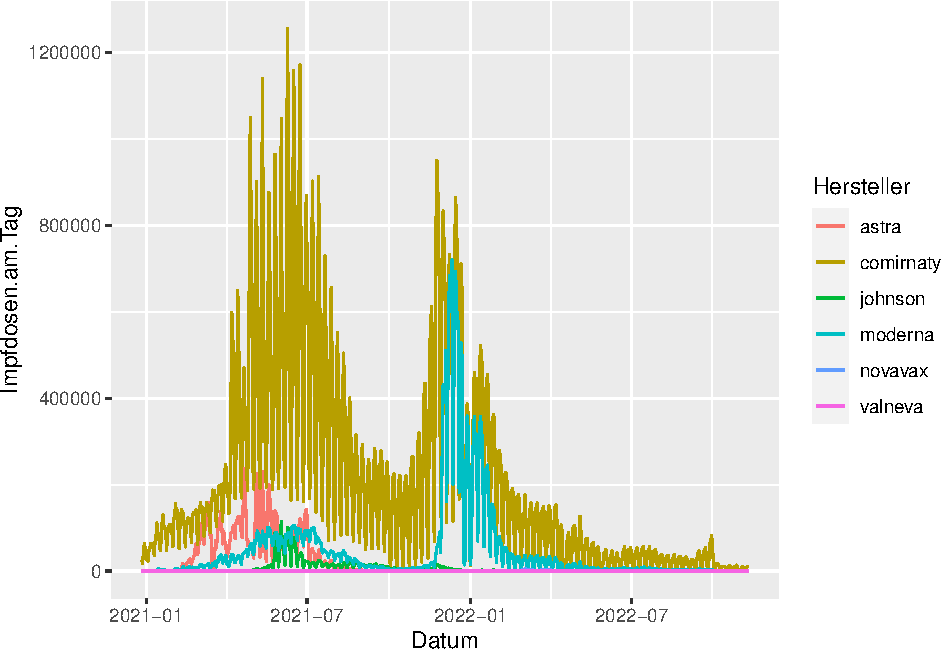
\includegraphics{Testat_1_Complete_files/figure-latex/unnamed-chunk-16-1.pdf}

\hypertarget{zeitverzug-auslieferung-bis-verimpfung}{%
\subsection{Zeitverzug Auslieferung bis
Verimpfung}\label{zeitverzug-auslieferung-bis-verimpfung}}

Es soll untersucht werden, wie schnell gelieferte Impfmengen der
einzelnen Impfstoffe auch verimpft wurden.

Es bietet sich dafür an, die akkumulierten Impfdosen mit den
akkumulierten Impflieferungen zeitlich plotten. Je größer die Lücke
zwischen der Liefermenge und der Impfungen ist, desto mehr Impfstoff
blieb liegen. Die Graphik soll Angaben für ganz Deutschland und nicht
für die einzelnen Bundesländer zeigen.

Hinweis: Auch hier ist eine Vorverarbeitung der Daten nötig.

Plotten Sie dies mit \emph{ggplot}:

\begin{Shaded}
\begin{Highlighting}[]
\CommentTok{\# Ihre Lösung:}

\NormalTok{deliv2 }\OtherTok{=} \FunctionTok{data.frame}\NormalTok{(deliv }\SpecialCharTok{|\textgreater{}} \FunctionTok{group\_by}\NormalTok{(impfstoff, date) }\SpecialCharTok{|\textgreater{}} \FunctionTok{summarise}\NormalTok{(}\AttributeTok{dosen =} \FunctionTok{sum}\NormalTok{(dosen)))}
\end{Highlighting}
\end{Shaded}

\begin{verbatim}
## `summarise()` has grouped output by 'impfstoff'. You can override using the
## `.groups` argument.
\end{verbatim}

\begin{Shaded}
\begin{Highlighting}[]
\DocumentationTok{\#\# gelieferte Dosen bis zum heutigen Tag vervollständigen}
\DocumentationTok{\#\# {-} besonders für Astra relevant, da Lieferstopp}
\NormalTok{last }\OtherTok{=}\NormalTok{ deliv2 }\SpecialCharTok{|\textgreater{}}
    \FunctionTok{group\_by}\NormalTok{(impfstoff) }\SpecialCharTok{|\textgreater{}}
    \FunctionTok{slice\_max}\NormalTok{(}\StringTok{\textquotesingle{}order\_by\textquotesingle{}}\OtherTok{=}\NormalTok{date, }\AttributeTok{n =} \DecValTok{1}\NormalTok{)}
\NormalTok{last}\SpecialCharTok{$}\NormalTok{date }\OtherTok{=} \FunctionTok{Sys.Date}\NormalTok{()}
\NormalTok{deliv3 }\OtherTok{=} \FunctionTok{rbind}\NormalTok{(deliv2, last)}
\DocumentationTok{\#\# ende}

\FunctionTok{ggplot}\NormalTok{() }\SpecialCharTok{+}
  \FunctionTok{geom\_line}\NormalTok{(}\FunctionTok{aes}\NormalTok{(}\AttributeTok{x=}\FunctionTok{as.Date}\NormalTok{(date), }\AttributeTok{y=}\FunctionTok{ave}\NormalTok{(dosen, impfstoff, }\AttributeTok{FUN=}\NormalTok{cumsum) , }\AttributeTok{group=}\NormalTok{impfstoff, }\AttributeTok{color=}\NormalTok{impfstoff), }
            \AttributeTok{linetype=}\StringTok{\textquotesingle{}dashed\textquotesingle{}}\NormalTok{, }\AttributeTok{data=}\NormalTok{deliv3) }\SpecialCharTok{+}
  \FunctionTok{labs}\NormalTok{(}\AttributeTok{x=}\StringTok{"Datum"}\NormalTok{, }\AttributeTok{y=}\StringTok{\textquotesingle{}Dosen\textquotesingle{}}\NormalTok{) }\SpecialCharTok{+}
  \FunctionTok{geom\_line}\NormalTok{(}\FunctionTok{aes}\NormalTok{(}\AttributeTok{x=}\FunctionTok{as.Date}\NormalTok{(Datum, }\StringTok{\textquotesingle{}\%d.\%m.\%Y\textquotesingle{}}\NormalTok{), }\AttributeTok{y=}\FunctionTok{ave}\NormalTok{(Impfdosen.am.Tag, Hersteller, }\AttributeTok{FUN=}\NormalTok{cumsum), }
                \AttributeTok{group=}\NormalTok{Hersteller, }\AttributeTok{color=}\NormalTok{Hersteller), }\AttributeTok{data=}\NormalTok{vacc2)}\SpecialCharTok{+}
  
  \FunctionTok{geom\_line}\NormalTok{(}\FunctionTok{aes}\NormalTok{(}\AttributeTok{x=}\FunctionTok{Sys.Date}\NormalTok{(), }\AttributeTok{y=}\DecValTok{0}\NormalTok{, }\AttributeTok{linetype=}\FunctionTok{factor}\NormalTok{(lt)), }\AttributeTok{data=}\FunctionTok{data.frame}\NormalTok{(}\AttributeTok{lt=}\DecValTok{1}\SpecialCharTok{:}\DecValTok{2}\NormalTok{)) }\SpecialCharTok{+}
\FunctionTok{scale\_linetype\_manual}\NormalTok{(}\AttributeTok{values=}\FunctionTok{c}\NormalTok{(}\StringTok{\textquotesingle{}solid\textquotesingle{}}\NormalTok{, }\StringTok{\textquotesingle{}dashed\textquotesingle{}}\NormalTok{), }\AttributeTok{name =}\StringTok{\textquotesingle{}Linetype\textquotesingle{}}\NormalTok{, }\AttributeTok{labels=}\FunctionTok{c}\NormalTok{(}\StringTok{\textquotesingle{}verimpft\textquotesingle{}}\NormalTok{,}\StringTok{\textquotesingle{}geliefert\textquotesingle{}}\NormalTok{))}
\end{Highlighting}
\end{Shaded}

\begin{verbatim}
## geom_path: Each group consists of only one observation. Do you need to adjust
## the group aesthetic?
\end{verbatim}

\includegraphics{Testat_1_Complete_files/figure-latex/unnamed-chunk-17-1.pdf}

\begin{Shaded}
\begin{Highlighting}[]
\CommentTok{\#+ scale\_y\_continuous(trans=\textquotesingle{}sqrt\textquotesingle{})}
\DocumentationTok{\#\#wurzelskala zieht die unteren Ergebnisse auseinander und macht es so ein bisschen anschaulicher}
\end{Highlighting}
\end{Shaded}


\end{document}
